\documentclass[a4paper]{article}
\usepackage{import}
%\usepackage[english,vietnam]{babel}
\usepackage[utf8]{inputenc}
%\usepackage[utf8]{inputenc}
%\usepackage[francais]{babel}
\usepackage{a4wide,amssymb,epsfig,latexsym,array,hhline,fancyhdr}
\usepackage[normalem]{ulem}
%\usepackage{soul}
\usepackage{listings}
\usepackage{colortbl}
\usepackage[makeroom]{cancel}
\usepackage{amsmath}
\usepackage{amsthm}
\usepackage{multicol,longtable,amscd}
\usepackage{diagbox}%Make diagonal lines in tables
\usepackage{booktabs}
\usepackage{alltt}
\usepackage[framemethod=tikz]{mdframed}% For highlighting paragraph backgrounds
\usepackage{caption,subcaption}

\usepackage{lastpage}
\usepackage[lined,boxed,commentsnumbered]{algorithm2e}
\usepackage{enumerate}
\usepackage{color}
\usepackage{graphicx}							% Standard graphics package
\usepackage{array}
\usepackage{tabularx, caption}
\usepackage{multirow}
\usepackage{multicol}
\usepackage{rotating}
\usepackage{graphics}
\usepackage{geometry}
\usepackage{setspace}
\usepackage{epsfig}
\usepackage{minted}
\usepackage{xcolor} % to access the named colour LightGray
\definecolor{LightGray}{gray}{0.9}
\usemintedstyle{emacs}
\usepackage{tikz}
\usetikzlibrary{graphs,graphs.standard}
\usetikzlibrary{arrows,snakes,backgrounds}
\usepackage[unicode]{hyperref}
\hypersetup{
    urlcolor=blue,
    linkcolor=black,
    citecolor=black,
    colorlinks=true,
    pdfpagemode=FullScreen,
    pdftitle={Convolution Operation Report},
} 
%\usepackage{pstcol} 								% PSTricks with the standard color package
%\usepackage{background}
%\backgroundsetup{contents=
\includegraphics{Images/hcmut.png}, scale=0.5, opacity=0.25, angle = 0}
\usepackage[normalem]{ulem}

\def\thesislayout{	% A4: 210 × 297
	\geometry{
		a4paper,
		total={160mm,240mm},  % fix over page
		left=30mm,
		top=30mm,
	}
}
\thesislayout

\usepackage{fancyhdr}
\setlength{\headheight}{40pt}
\pagestyle{fancy}
\fancyhead{} % clear all header fields
\fancyhead[L]{
 \begin{tabular}{rl}
    \begin{picture}(25,15)(0,0)
    \put(0,-8){
\includegraphics[width=8mm, height=8mm]{Images/hcmut.png}}
    %\put(0,-8){\epsfig{width=10mm,figure=hcmut.eps}}
   \end{picture}&
	%
\includegraphics[width=8mm, height=8mm]{hcmut.png} & %
	\begin{tabular}{l}
		\textbf{\textcolor{blue}{\bf \ttfamily Ho Chi Minh City University of Technology}}\\
		\textbf{\textcolor{blue}{\bf \ttfamily Faculty of Computer Science and Engineering}}
	\end{tabular} 	
 \end{tabular}
}
\fancyhead[R]{
	\begin{tabular}{l}
		\tiny \bf \\
		\tiny \bf 
	\end{tabular}  }
\fancyfoot{} % clear all footer fields
\fancyfoot[L]{\scriptsize \ttfamily Truong Gia Ky Nam - 2352787}
\fancyfoot[R]{\scriptsize \ttfamily Page {\thepage}/\pageref{LastPage}}
\renewcommand{\headrulewidth}{0.3pt}
\renewcommand{\footrulewidth}{0.3pt}


%%%
\setcounter{secnumdepth}{4}
\setcounter{tocdepth}{3}
\makeatletter
\newcounter {subsubsubsection}[subsubsection]
\renewcommand\thesubsubsubsection{\thesubsubsection .\@alph\c@subsubsubsection}
\newcommand\subsubsubsection{\@startsection{subsubsubsection}{4}{\z@}%
                                     {-3.25ex\@plus -1ex \@minus -.2ex}%
                                     {1.5ex \@plus .2ex}%
                                     {\normalfont\normalsize\bfseries}}
\newcommand*\l@subsubsubsection{\@dottedtocline{3}{10.0em}{4.1em}}
\newcommand*{\subsubsubsectionmark}[1]{}
\makeatother

\sloppy
\captionsetup[figure]{labelfont={small,bf},textfont={small,it},belowskip=-1pt,aboveskip=-9pt}
%space remove between caption, figure, and text
\captionsetup[table]{labelfont={small,bf},textfont={small,it},belowskip=-1pt,aboveskip=7pt}
%space remove between caption, table, and text

%\floatplacement{figure}{H}%forced here float placement automatically for figures
%\floatplacement{table}{H}%forced here float placement automatically for table
%the following settings (11 lines) are to remove white space before or after the figures and tables
%\setcounter{topnumber}{2}
%\setcounter{bottomnumber}{2}
%\setcounter{totalnumber}{4}
%\renewcommand{\topfraction}{0.85}
%\renewcommand{\bottomfraction}{0.85}
%\renewcommand{\textfraction}{0.15}
%\renewcommand{\floatpagefraction}{0.8}
%\renewcommand{\textfraction}{0.1}
\setlength{\floatsep}{5pt plus 2pt minus 2pt}
\setlength{\textfloatsep}{5pt plus 2pt minus 2pt}
\setlength{\intextsep}{10pt plus 2pt minus 2pt}

\thesislayout



\begin{document}
\begin{titlepage}
\begin{center}
\textbf{\Large VIETNAM NATIONAL UNIVERSITY HO CHI MINH CITY} \\

\vspace{7pt}
\textbf{\Large HO CHI MINH CITY UNIVERSITY OF TECHNOLOGY} \\

\vspace{7pt}
\textbf{\Large FACULTY OF COMPUTER SCIENCE AND ENGINEERING}
\end{center}

\vspace{1cm}

\begin{figure}[h!]
\begin{center}

\includegraphics[width=3cm]{Images/hcmut.png}
\end{center}
\end{figure}

\vspace{1cm}


\begin{center}
\begin{tabular}{ccc}
	\multicolumn{3}{l}{\textbf{{\Large \textcolor{blue}{COMPUTER ARCHITECTURE LAB (CO2008)}}}}\\
	~~\\
	\arrayrulecolor{blue}\hline
	\\
	\multicolumn{3}{l}{\textbf{{\Large \textcolor{blue}{Assignment} }}}\\
	\\
	
	\multicolumn{3}{c}{\textbf{{\huge \textcolor{blue}{CONVOLUTION OPERATION}}}}\\
	\\

	\arrayrulecolor{blue}\hline \\ \\

    \multicolumn{1}{r}{\textbf{\Large Instructors:}} & \multicolumn{2}{l}{\Large Nguyen Thanh Loc} \\ \\

    \\ \\

    \multicolumn{1}{r}{\Large \textbf{Author:}} & \multicolumn{2}{l}{\Large Truong Gia Ky Nam} \\ \\

	\multicolumn{1}{r}{\Large \textbf{Class:}} & \multicolumn{2}{l}{\Large CC04} \\ \\

    \multicolumn{1}{r}{\Large \textbf{ID:}} & \multicolumn{2}{l}{\Large 2352787} \\ \\

    \multicolumn{1}{r}{\Large \textbf{Email:}} & \multicolumn{2}{l}{\Large nam.truonggiaky@hcmut.edu.vn} \\ \\
\end{tabular}
\end{center}

\vspace{4cm}

\begin{center}
{\textbf{\Large Ho Chi Minh City, November 2024}}
\end{center}
\end{titlepage}

\thispagestyle{empty}
\setcounter{page}{-1}
\newpage
\begin{abstract}
    \noindent The convolution operation is a fundamental technique in digital signal processing and computer vision used for various applications such as image filtering, feature detection, and edge detection. This process involves overlaying a smaller matrix (kernel or filter) on a larger matrix (input data) and computing a weighted sum of the overlapping values. The result is stored in an output matrix, effectively transforming the input according to the properties of the kernel. In the context of MIPS assembly programming, implementing convolution involves manually handling matrix data, iterating over elements, performing multiplications and additions, and managing memory storage—all within the constraints of low-level instruction sets. The assignment will demonstrate the ability to break down complex mathematical operations into MIPS assembly code, showcasing proficiency in logical flow, register management, and computational efficiency in the MARS simulator environment.
\end{abstract}
\newpage

\setcounter{page}{0}
\thispagestyle{empty}
\newpage
\tableofcontents
\newpage

%\thispagestyle{empty}
\section{Introduction}
This report describes the implementation of a Convolution Operation using MIPS
assembly language. The convolution process is widely used in digital image processing
and deep learning, particularly for tasks like feature extraction and image filtering. This
program performs a convolution operation on an input matrix (image) with a kernel
(filter) and outputs the result to a file. The implementation considers constraints like
input validation, padding, and kernel size compatibility with the input matrix 
\section{Convolution operation}
The convolution operation is a fundamental mathematical process widely used in signal processing, image processing, and deep learning, particularly in convolutional neural networks (CNNs). At its core, convolution involves the sliding of a filter or kernel over an input data structure, such as a one-dimensional signal or a two-dimensional image, to produce an output known as the feature map. This operation effectively transforms the input by highlighting certain patterns or features, such as edges or textures in an image, making it essential for feature extraction in computer vision tasks.\\ \\
In the case of image processing, convolution works by positioning a small matrix called a kernel over a region of the image, multiplying corresponding values, and summing the results to produce a single output pixel in the feature map. This process is repeated as the kernel slides across the entire image, creating a matrix that encodes information about local patterns. By applying different kernels, such as those for edge detection, sharpening, or blurring, convolution allows for various types of image transformations and analysis. The size and values of the kernel determine the type of feature that is emphasized, while parameters like stride and padding control the movement and preservation of image dimensions.
   
\section{Explanation of the Algorithm}
\begin{figure}[!h]
\centering
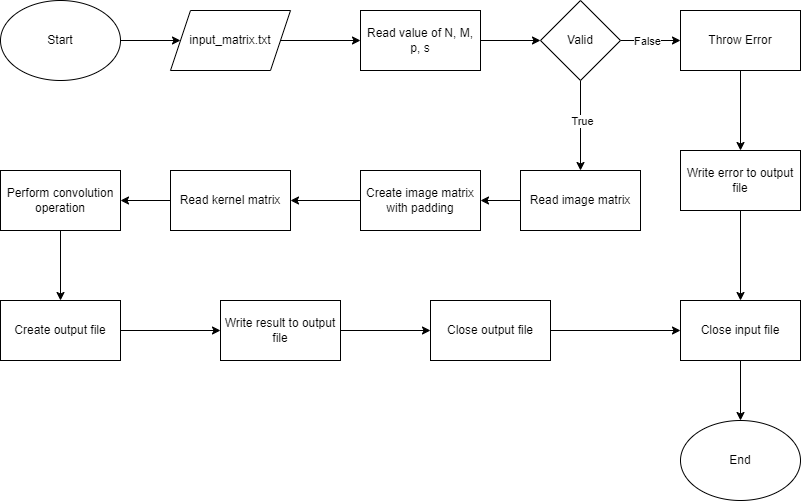
\includegraphics[scale=0.5]{Images/flowchart.png}
\end{figure}
To see the full source code, take a look at the file: \textit{assignment.asm}\\ \\
\subsection{Overview}
The program is structured into several logical sections to ensure efficient execution:
\begin{enumerate}
	\item Input File Handling
	\begin{itemize}
		\item Reads an input file (input matrix.txt) containing matrix dimensions, padding,
		stride, and the matrix data.
		\item Handles potential errors such as invalid or out-of-bound inputs.
	\end{itemize}
	\item Validation of Inputs
	\begin{itemize}
		\item Validates dimensions of the matrix, kernel size, padding, and stride against
		defined constraints.
		\item Generates error messages for: kernel size larger than image; invalid constraints
	\end{itemize}
	\item Padding the Input Matrix
	\begin{itemize}
		\item Adds zero-padding around the input matrix based on the specified padding
		size (p).
		\item The padded matrix dimensions are calculated as N + 2P.
	\end{itemize}
	\item Kernel and Matrix Reading
	\begin{itemize}
		\item Reads the kernel (filter) matrix from the input.
		\item Converts string inputs into floating-point numbers using a custom parser.
	\end{itemize}
	\item Convolution Operation
	\begin{itemize}
		\item Iterates over the padded image matrix with a specified stride (s) to compute
		the output matrix.
		\item Performs element-wise multiplication of the kernel and corresponding image
		sub-matrix, followed by summation.
	\end{itemize}
	\item Output File Handling
	\begin{itemize}
		\item Writes the resulting output matrix to output matrix.txt.
		\item Outputs the values in a formatted way, including floating-point conversion.
	\end{itemize}
	\item Error Handling
	\begin{itemize}
		\item Detects and reports specific errors like invalid inputs, kernel larger than the
		image, and overflow issues.
		\item Ensures graceful program termination with error messages when constraints
		are violated.
	\end{itemize}
\end{enumerate}
\subsection{Detail Explanation}
First, a reading pointer will be initialized for reading data in the input file. The pointer will read the first line to store values of the image size, the kernel size, the padding and the stride. After get all these initial value, it will check if those values are in the given constrains or not. After the first 4 values are valid, the size of the padded image and the output matrix size are calculated by using the formula 
\begin{equation*}
	N_{padding} = N_{image} + 2 \times P
\end{equation*}
where $N_{image}$ is the size of the image matrix, P is the value of padding and $N_{padding}$ is the size of the padding image matrix. Also, the output matrix size is calculated by using the formula
\begin{equation*}
	N_{output} = \frac{N_{image} + 2 \times P - N_{kernel}}{S} + 1
\end{equation*} 
where $N_{kernel}$ is the size of the filter matrix and S is the stride value.\\ \\
Next, pointer will move to read the data for the image matrix. To read and store value as a 2-dimensional matrix, initialize a 2 running variable i and j (represent for row and column index), for each value read in the input file, it will be store in the correct position of the 2D matrix. The address for elements image[i][j] is calculated by
\begin{equation*}
	Image[i][j] = BaseAddressOfImageMatrix + i \times N + j 
\end{equation*} 
When the correct position is found, the pointer will iterate through each digit and the dot to produce the floating-point number. The process is taken place by convert each characters to digit and combine them. Before the decimal point, that is the integer part, store the it in the first register. After the decimal point, that is the decimal part, is stored in another register. When reaching the space character, these two values are combine together to make the complete float number. The process of calculating matrix address and read floating value continue until all values of the image matrix are read. The pointer continue to move to the kernel data to read and store in the kernel matrix.\\ \\
After reading data for image and kernel matrix, the padded image matrix is created with the size $N_{padding}$ by putting the image matrix in the center of the padding image matrix. To put the image matrix to the center of the padded image matrix, for each element image[i][j], put it at the position $padded\_image$[i + p][j + p] where p is the stride value.\\ \\
When everything is ready, the convolution operation begin. To perform the convolution operation, loop through each cell of the output matrix. At each cell, extract corresponding data in the image and the kernel and calculate the result and store it in the output matrix. Repeat the process until all elements in the output matrix are filled. Finally, from the output matrix, write each element to the output file. It begins by clearing the buffer for storing the result. If the number is negative, it adds a negative sign and adjusts the value accordingly. The function extracts the integer and fractional parts of the number, using $int\_to\_string$ to convert each part into a string, with a decimal point separating them. It handles edge cases where either part equals zero and ensures the fractional part is padded with leading zeros to maintain four decimal places. The final string is shifted appropriately to include the negative sign if needed and null-terminated to mark the end.  
\section{Sample output}
Input 1:
\begin{figure}[!h]
\centering
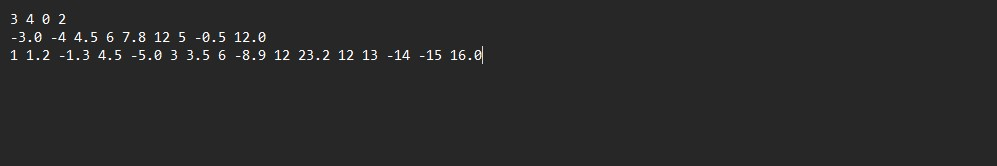
\includegraphics[scale=0.5]{Images/i1.jpg}
\end{figure}\\
Output 1:
\begin{figure}[!h]
	\centering
	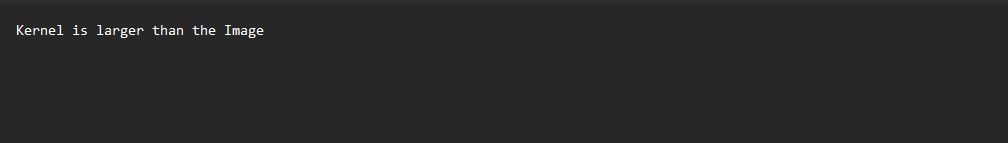
\includegraphics[scale=0.5]{Images/o1.jpg}
\end{figure}\\
Input 2:
\begin{figure}[!h]
	\centering
	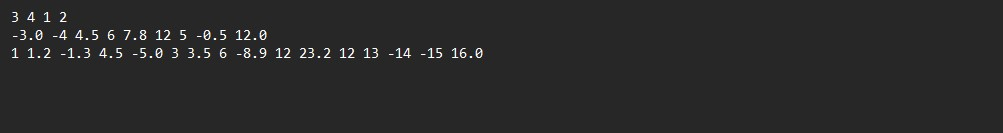
\includegraphics[scale=0.5]{Images/i2.jpg}
	\end{figure}\\
\pagebreak
Output 2:
\begin{figure}[!h]
	\centering
	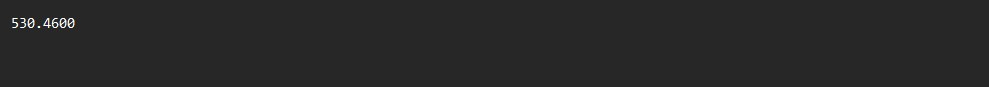
\includegraphics[scale=0.5]{Images/o2.jpg}
	\end{figure}\\
Input 3:
\begin{figure}[!h]
	\centering
	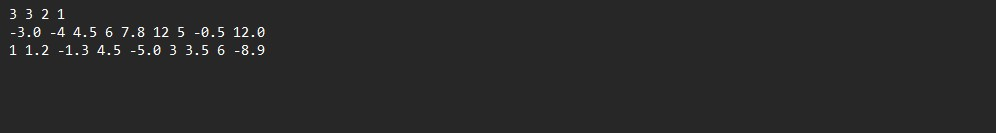
\includegraphics[scale=0.5]{Images/i3.jpg}
	\end{figure}\\
Output 3:
\begin{figure}[!h]
	\centering
	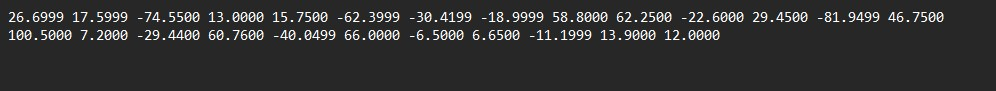
\includegraphics[scale=0.5]{Images/o3.jpg}
	\end{figure}\\
Input 4:
\begin{figure}[!h]
	\centering
	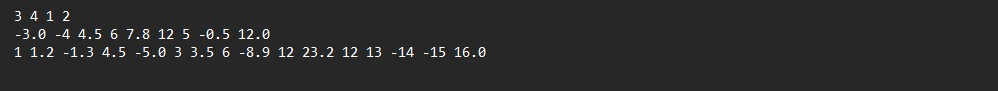
\includegraphics[scale=0.5]{Images/i4.jpg}
	\end{figure}\\
Output 4:
\begin{figure}[!h]
	\centering
	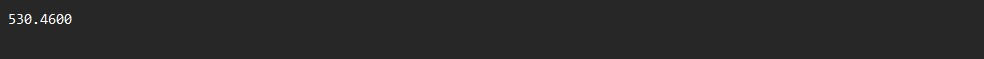
\includegraphics[scale=0.5]{Images/o4.jpg}
	\end{figure}\\
Input 5:
\begin{figure}[!h]
	\centering
	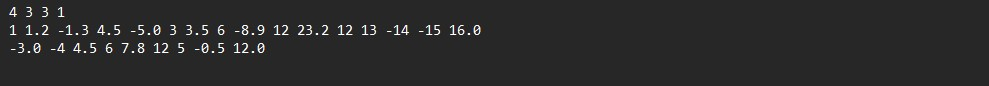
\includegraphics[scale=0.5]{Images/i5.jpg}
	\end{figure}\\
Output 5:
\begin{figure}[!h]
	\centering
	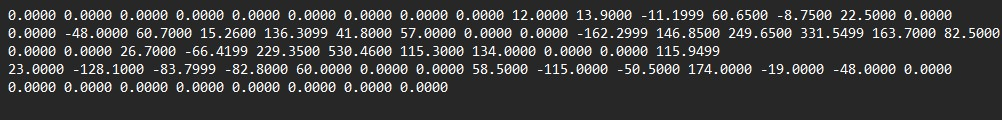
\includegraphics[scale=0.5]{Images/o5.jpg}
	\end{figure}\\
Input 6:
\begin{figure}[!h]
	\centering
	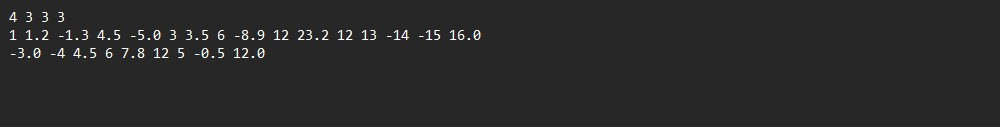
\includegraphics[scale=0.5]{Images/i6.jpg}
	\end{figure}\\
Output 6:
\begin{figure}[!h]
	\centering
	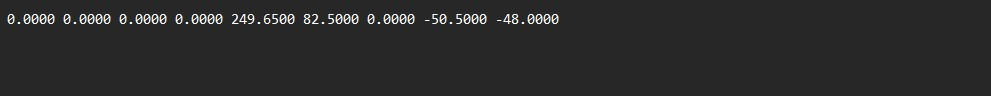
\includegraphics[scale=0.5]{Images/o6.jpg}
	\end{figure}\\
Input 7:
\begin{figure}[!h]
	\centering
	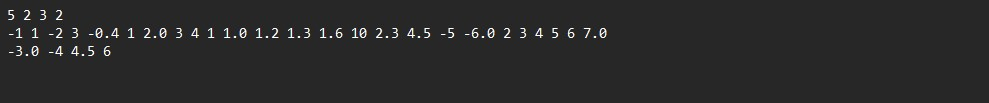
\includegraphics[scale=0.5]{Images/i7.jpg}
	\end{figure}\\
\pagebreak
Output 7:
\begin{figure}[!h]
	\centering
	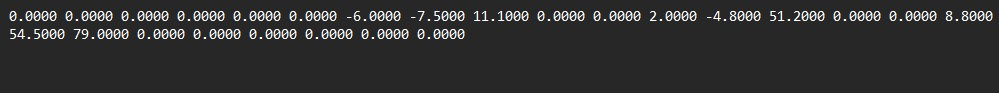
\includegraphics[scale=0.5]{Images/o7.jpg}
	\end{figure}\\
Input 8:
\begin{figure}[!h]
	\centering
	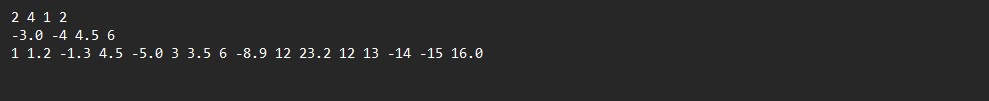
\includegraphics[scale=0.5]{Images/i8.jpg}
	\end{figure}\\
Output 8:
\begin{figure}[!h]
	\centering
	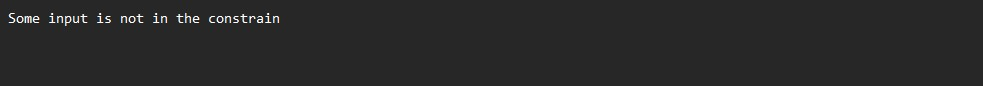
\includegraphics[scale=0.5]{Images/o8.jpg}
	\end{figure}\\
\end{document}

